\section{Geometry and the finite construction}\label{sec:construction}

We first fix the area scale against which the covering will be measured.
We then specify every triangle and every axis in the finite covering.
The projection calculation is the facet-area-vector form of Cauchy's
projection formula; see \cite[p.~83, equation~(1)]{Martini1991} for its
projection-body formulation. We include the face-by-face proof for this tetrahedron.

\begin{lemma}\label{lem:projection-minimum}
For the tetrahedron \eqref{eq:tetrahedron}, $A_{\min}(K)=H$.
\end{lemma}
\begin{proof}
The outward face area vectors (unit normal multiplied by face area) are
\[
 (0,\pm H,-1),\qquad (\pm H,0,1).
\]
Indeed, the supporting planes are $\pm Hy-z=0$ and
$\pm Hx+z=H$. The displayed outward normals have length $\sqrt3$,
which is the area of each equilateral face of side length $2$.
For a unit vector $u$, the faces with positive scalar product against $u$ project to partition the shadow, apart from the projections of edges and parallel faces, which have area zero.
They give the forward endpoints of the chords parallel to $u$.
The projected area of a face with area vector $N$ is $|N\cdot u|$,
as follows by projecting its two edge vectors and taking their cross product.
The sum of the four area vectors is zero. Thus the shadow area is half the sum of their absolute scalar products with $u$, namely
\[
 A(u)=\max(H|u_x|,|u_z|)+\max(H|u_y|,|u_z|).
\]
Put $U=\max(|u_x|,|u_z|/H)$ and $V=\max(|u_y|,|u_z|/H)$.
Since $H^2=2$,
\[
 (U+V)^2\ge |u_x|^2+|u_y|^2+2|u_z|^2/H^2=1.
\]
Here $U^2\ge|u_x|^2$, $V^2\ge|u_y|^2$ and
$UV\ge|u_z|^2/H^2$ account for the three terms separately.
Hence $A(u)=H(U+V)\ge H$, with equality at $u=(1,0,0)$.
\end{proof}

At zero tilt, the part $t\le1/2$ is covered by an $x$-parallel cylinder and the part $t\ge1/2$ by a $y$-parallel cylinder.
Each perpendicular base is a triangle of area $H/4$.
The lower intercept triangle can be parametrized as
\[
 (0,qt_0,Ht_0),\qquad -1\le q\le1,\quad 0\le t_0\le1/2.
\]
Here $q$ is a slope parameter: for $t_0>0$ it is the second coordinate
divided by $t_0$.
We call the intervals of $q$ angular sectors. The radial height $t_0$
is the third physical coordinate divided by $H$, rather than Euclidean
distance from the tip. The upper intercept triangle is similarly
$(ps_0,0,H(1-s_0))$, with $-1\le p\le1$ and $0\le s_0\le1/2$.
We now perturb a finite subdivision of these triangles.

Fix a positive tilt parameter $\eps$, and put
\begin{equation}\label{eq:parameters}
 \eta=\frac1{1000},\qquad
 n=\left\lceil\frac2{\eps^2}\right\rceil,\qquad
 \Delta=\frac2n,\qquad q_j=-1+j\Delta\quad(0\le j\le n).
\end{equation}
In particular $\Delta\le\eps^2$.
To make adjacent tilted sectors meet, prescribe the displacement of the
boundary with angular parameter $q$ by
\[
 \phi(q)=\frac{1-q^2}{4}\qquad(-1\le q\le1).
\]
The endpoint values $\phi(-1)=\phi(1)=0$ will keep the outer angular
sides in the fixed planes $y=-t$ and $y=t$.
For real $\alpha,\beta$, the lines with direction
$(1,\eps\alpha,H\eps\beta)$ through the points
$(0,qt_0,Ht_0)$, $t_0\ge0$, lie in the plane
\[
 y=qt+\eps x(\alpha-q\beta).
\]
Thus neighboring angular sides will lie in the same plane if both axes
use the value $\phi(q)$ there. On the interval $[q_j,q_{j+1}]$, solve the
two endpoint equations $\alpha_j-q\beta_j=\phi(q)$. This gives
\begin{equation}\label{eq:axis-coefficients}
 \alpha_j=\frac{1+q_jq_{j+1}}4,
 \qquad \beta_j=\frac{q_j+q_{j+1}}4
 \qquad(0\le j<n),
\end{equation}
and hence the exact matching identities
\begin{equation}\label{eq:shared-boundaries}
 \alpha_j-q\beta_j=\frac{1-q^2}{4}
 \qquad(q=q_j\text{ or }q=q_{j+1}).
\end{equation}

The choice of parabola also anticipates the radial estimate. At zero
tilt, the ray of slope $q$ meets the middle section at $y=q/2$.
The lower intercept height
$t_0=t-\eps x\beta_j$ should have first-order shift $-\eps xy$.
This suggests $\beta_j\simeq q/2$. The endpoint equations make
$\beta_j$ the negative secant slope of $\phi$, so their limiting
relation is $\phi'(q)=-q/2$. Together with the two endpoint conditions,
this gives $\phi(q)=(1-q^2)/4$. The finite identities above, rather
than this motivation, will be used in the proof.

We also enlarge each sector slightly beyond its original radial cutoff
$1/2$. Define
\begin{equation}\label{eq:cutoffs}
 d(q)=\frac{q^2(1+q^2)}{16},\qquad
 M_j=\eta+\max_{q_j\le q\le q_{j+1}}d(q),\qquad
 T_j=\frac12+\eps^2M_j.
\end{equation}
The function $d$ bounds the quadratic loss in the overlap of the two
families; its role is made explicit in the coverage argument below.
For later estimates, note that
\begin{equation}\label{eq:coefficient-bounds}
 0\le\alpha_j\le\tfrac12,\qquad |\beta_j|\le\tfrac12,
 \qquad \eta\le M_j\le\tfrac18+\eta.
\end{equation}

Our intercept triangles and direction vectors are
\begin{align}
 P_j&=\{(0,y_0,Ht_0):0\le t_0\le T_j,
                  \ q_jt_0\le y_0\le q_{j+1}t_0\},
 &v_j&=(1,\eps\alpha_j,H\eps\beta_j),\label{eq:first-family}\\
 Q_j&=\{(x_0,0,H(1-s_0)):0\le s_0\le T_j,
                  \ q_js_0\le x_0\le q_{j+1}s_0\},
 &w_j&=(-\eps\alpha_j,1,H\eps\beta_j).\label{eq:second-family}
\end{align}
Use the $2n$ cylinders
\[
 P_j+\R v_j,\qquad Q_j+\R w_j\qquad(0\le j<n).
\]
To express them with perpendicular bases, project each intercept triangle onto the linear plane perpendicular to its direction and normalize that direction.
Projection along the axis does not change the cylinder:
$P+\R v=\pi_{v^\perp}P+\R v$.
Moreover, it is injective on either intercept plane because the corresponding normal component of $v_j$ or $w_j$ is $1$.
Thus each actual base is a compact nondegenerate triangle, with finite area.

Figure~\ref{fig:construction} shows the original covering and the angular
matching after the tilt. In a fixed plane $x=X$, the neighboring sectors
start at different translated vertices
$V_i=(\eps X\alpha_i,\eps X\beta_i)$ in $(y,t)$ coordinates, but their
sides at a shared value of $q$ lie on the same line. Thus the matching
concerns the supporting planes of the sides; the radial extents still
have to be checked.

\begin{figure}[!htb]
  \centering
  \begin{minipage}[t]{0.48\linewidth}
    \centering
    {\small\textbf{(a)} The zero-tilt geometry, $\eps=0$}\par\smallskip
    \begin{tikzpicture}[x=0.205\linewidth,y=0.205\linewidth,
      font=\scriptsize,line cap=round,line join=round]
      \coordinate (A) at (-1.8,0.4);   %
      \coordinate (B) at (1.8,-0.4);   %
      \coordinate (C) at (-0.95,2.45); %
      \coordinate (D) at (0.95,3.35);  %
      \coordinate (AC) at (-1.375,1.425);
      \coordinate (BC) at (0.425,1.025);
      \coordinate (BD) at (1.375,1.475);
      \coordinate (AD) at (-0.425,1.875);
      \fill[black!3] (A)--(B)--(D)--(C)--cycle;
      \draw[black!45,densely dashed] (A)--(D);
      \fill[blue!9] (AC)--(BC)--(BD)--(AD)--cycle;
      \draw[black!55,thin] (AC)--(BC)--(BD)--(AD)--cycle;
      \draw[black!65] (A)--(C)--(D)--(B)--cycle (B)--(C);
      \draw[blue!65!black,very thick] (A)--(B);
      \draw[orange!80!black,very thick] (C)--(D);
      \draw[->,blue!65!black,thick] (-1.121,0.821)--(0.931,0.365);
      \draw[->,blue!65!black,thick] (-0.679,1.232)--(0.869,0.888);
      \draw[->,orange!80!black,thick] (-0.352,1.970)--(0.712,2.474);
      \draw[->,orange!80!black,thick] (-0.5885,1.8185)--(0.2285,2.2055);
      \node[blue!65!black,anchor=north] at (0.48,0.35) {$x$};
      \node[orange!80!black,anchor=south west] at (0.70,2.48) {$y$};
      \node[fill=white,inner sep=1.3pt] at (0,1.44) {$t=\tfrac12$};
      \node at (-1.50,-0.13) {$(-1,0,0)$};
      \node at (1.50,-0.83) {$(1,0,0)$};
      \node at (-1.44,2.94) {$(0,-1,H)$};
      \node at (1.04,3.81) {$(0,1,H)$};
      \path[use as bounding box] (-2.38,-0.99) rectangle (2.38,4.00);
    \end{tikzpicture}\par
    {\scriptsize Physical coordinates $(x,y,Ht)$; $H=\sqrt{2}$.}
  \end{minipage}\hfill
  \begin{minipage}[t]{0.49\linewidth}
    \centering
    {\small\textbf{(b)} Matching after the tilt, $x=X$}\par\smallskip
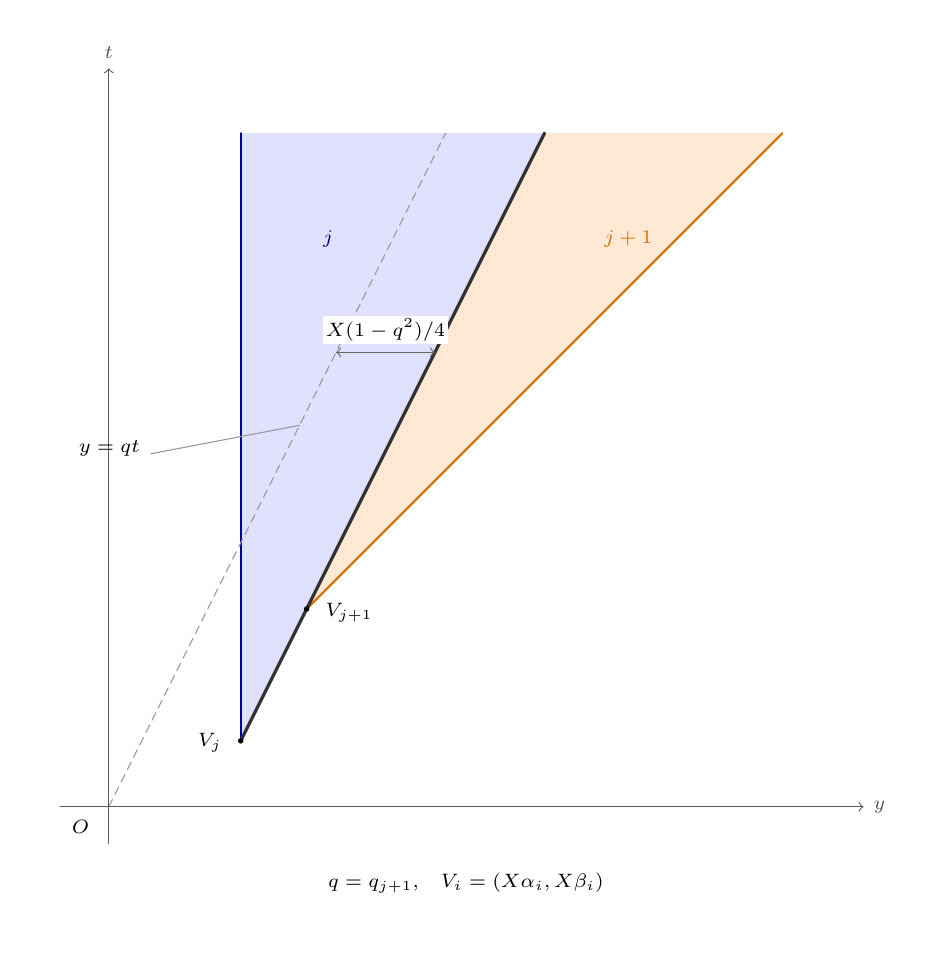
\begin{tikzpicture}[x=0.85\linewidth,y=0.85\linewidth,
  font=\scriptsize,line cap=round,line join=round]
  \coordinate (A) at (.1625,.08125);
  \coordinate (B) at (.24375,.24375);
  \coordinate (Ltop) at (.1625,.83);
  \coordinate (Mtop) at (.536875,.83);
  \coordinate (Rtop) at (.83,.83);
  \fill[blue!12] (A)--(Ltop)--(Mtop)--cycle;
  \fill[orange!17] (B)--(Mtop)--(Rtop)--cycle;
  \draw[blue!65!black,thick] (A)--(Ltop);
  \draw[orange!85!black,thick] (B)--(Rtop);
  \draw[black!80,very thick] (A)--(Mtop);
  \draw[black!40,densely dashed] (0,0)--(.415,.83);
  \draw[<->,black!60] (.28,.56)--(.401875,.56);
  \node[fill=white,inner sep=1pt,anchor=south] at (.3409375,.57)
    {$\eps X(1-q^2)/4$};
  \draw[->,black!65] (-.06,0)--(.93,0) node[right] {$y$};
  \draw[->,black!65] (0,-.045)--(0,.91) node[above] {$t$};
  \node[anchor=north east] at (-.012,-.005) {$O$};
  \fill (A) circle[radius=1pt];
  \fill (B) circle[radius=1pt];
  \node[anchor=east] at (.151,.079) {$V_j$};
  \node[anchor=west] at (.255,.239) {$V_{j+1}$};
  \node[blue!65!black] at (.27,.70) {$j$};
  \node[orange!85!black] at (.64,.70) {$j+1$};
  \node[anchor=south east,align=right] at (.05,.42) {$y=qt$};
  \draw[black!40,thin] (.052,.435)--(.235,.47);
  \node[anchor=north,align=center] at (.44,-.07)
    {$q=q_{j+1}$,\quad $V_i=(\eps X\alpha_i,\eps X\beta_i)$};
  \path[use as bounding box] (-.10,-.15) rectangle (1,.96);
\end{tikzpicture}\par
{\scriptsize The common supporting line is $y=qt+\eps X(1-q^2)/4$.}

  \end{minipage}
  \caption{(a) At zero tilt, cylinders parallel to the two opposite edges cover the lower and upper halves of $K$.
  (b) In the plane $x=X$, neighboring angular sectors have distinct translated vertices $V_j$ and $V_{j+1}$, but their sides at $q=q_{j+1}$ lie on the same line $y=qt+\eps X(1-q^2)/4$.
  The dashed line is $y=qt$, its zero-tilt position. Tilt and sector widths are exaggerated. Radial cutoffs are omitted; the colored regions end at the boundary of the displayed window.}
  \label{fig:construction}
\end{figure}

